\begin{Ueberlieferung}% 
{\textit{L}}Konzept: LH XXXVII 5 Bl. 135-136. 1 Bog. 4\textsuperscript{o}. 3 S. einspaltig. Bl. 136~v\textsuperscript{o} leer. Ein
Wasserzeichen mittig. \\%
Cc 2, Nr. 541
\end{Ueberlieferung}
%
\begin{Datierungsgruende}%
Das vorliegende Stück ist auf Pariser Papier verfasst.
Das Wasserzeichen lässt sich jedoch nicht weiter chronologisch zuordnen.
In der Marginalie auf der ersten Seite des Bogens bemerkt Leibniz selbst,
er habe noch nicht verstanden, was das Baryzentrum sei,
als er diesen Text geschrieben habe.
Dies weist auf eine eher frühe Entstehung hin.
Die thematische Verwandschaft mit dem Stück N.~42
% 037_04_049 = Demonstratio de trabis aequilibrio brachiis inaequalibus 
legt eine Datierung auf denselben Zeitraum nahe.
\end{Datierungsgruende}
%
\pstartfirst%
%\begin{wrapfigure}{l}{0.5\textwidth}
%\vspace{-4mm}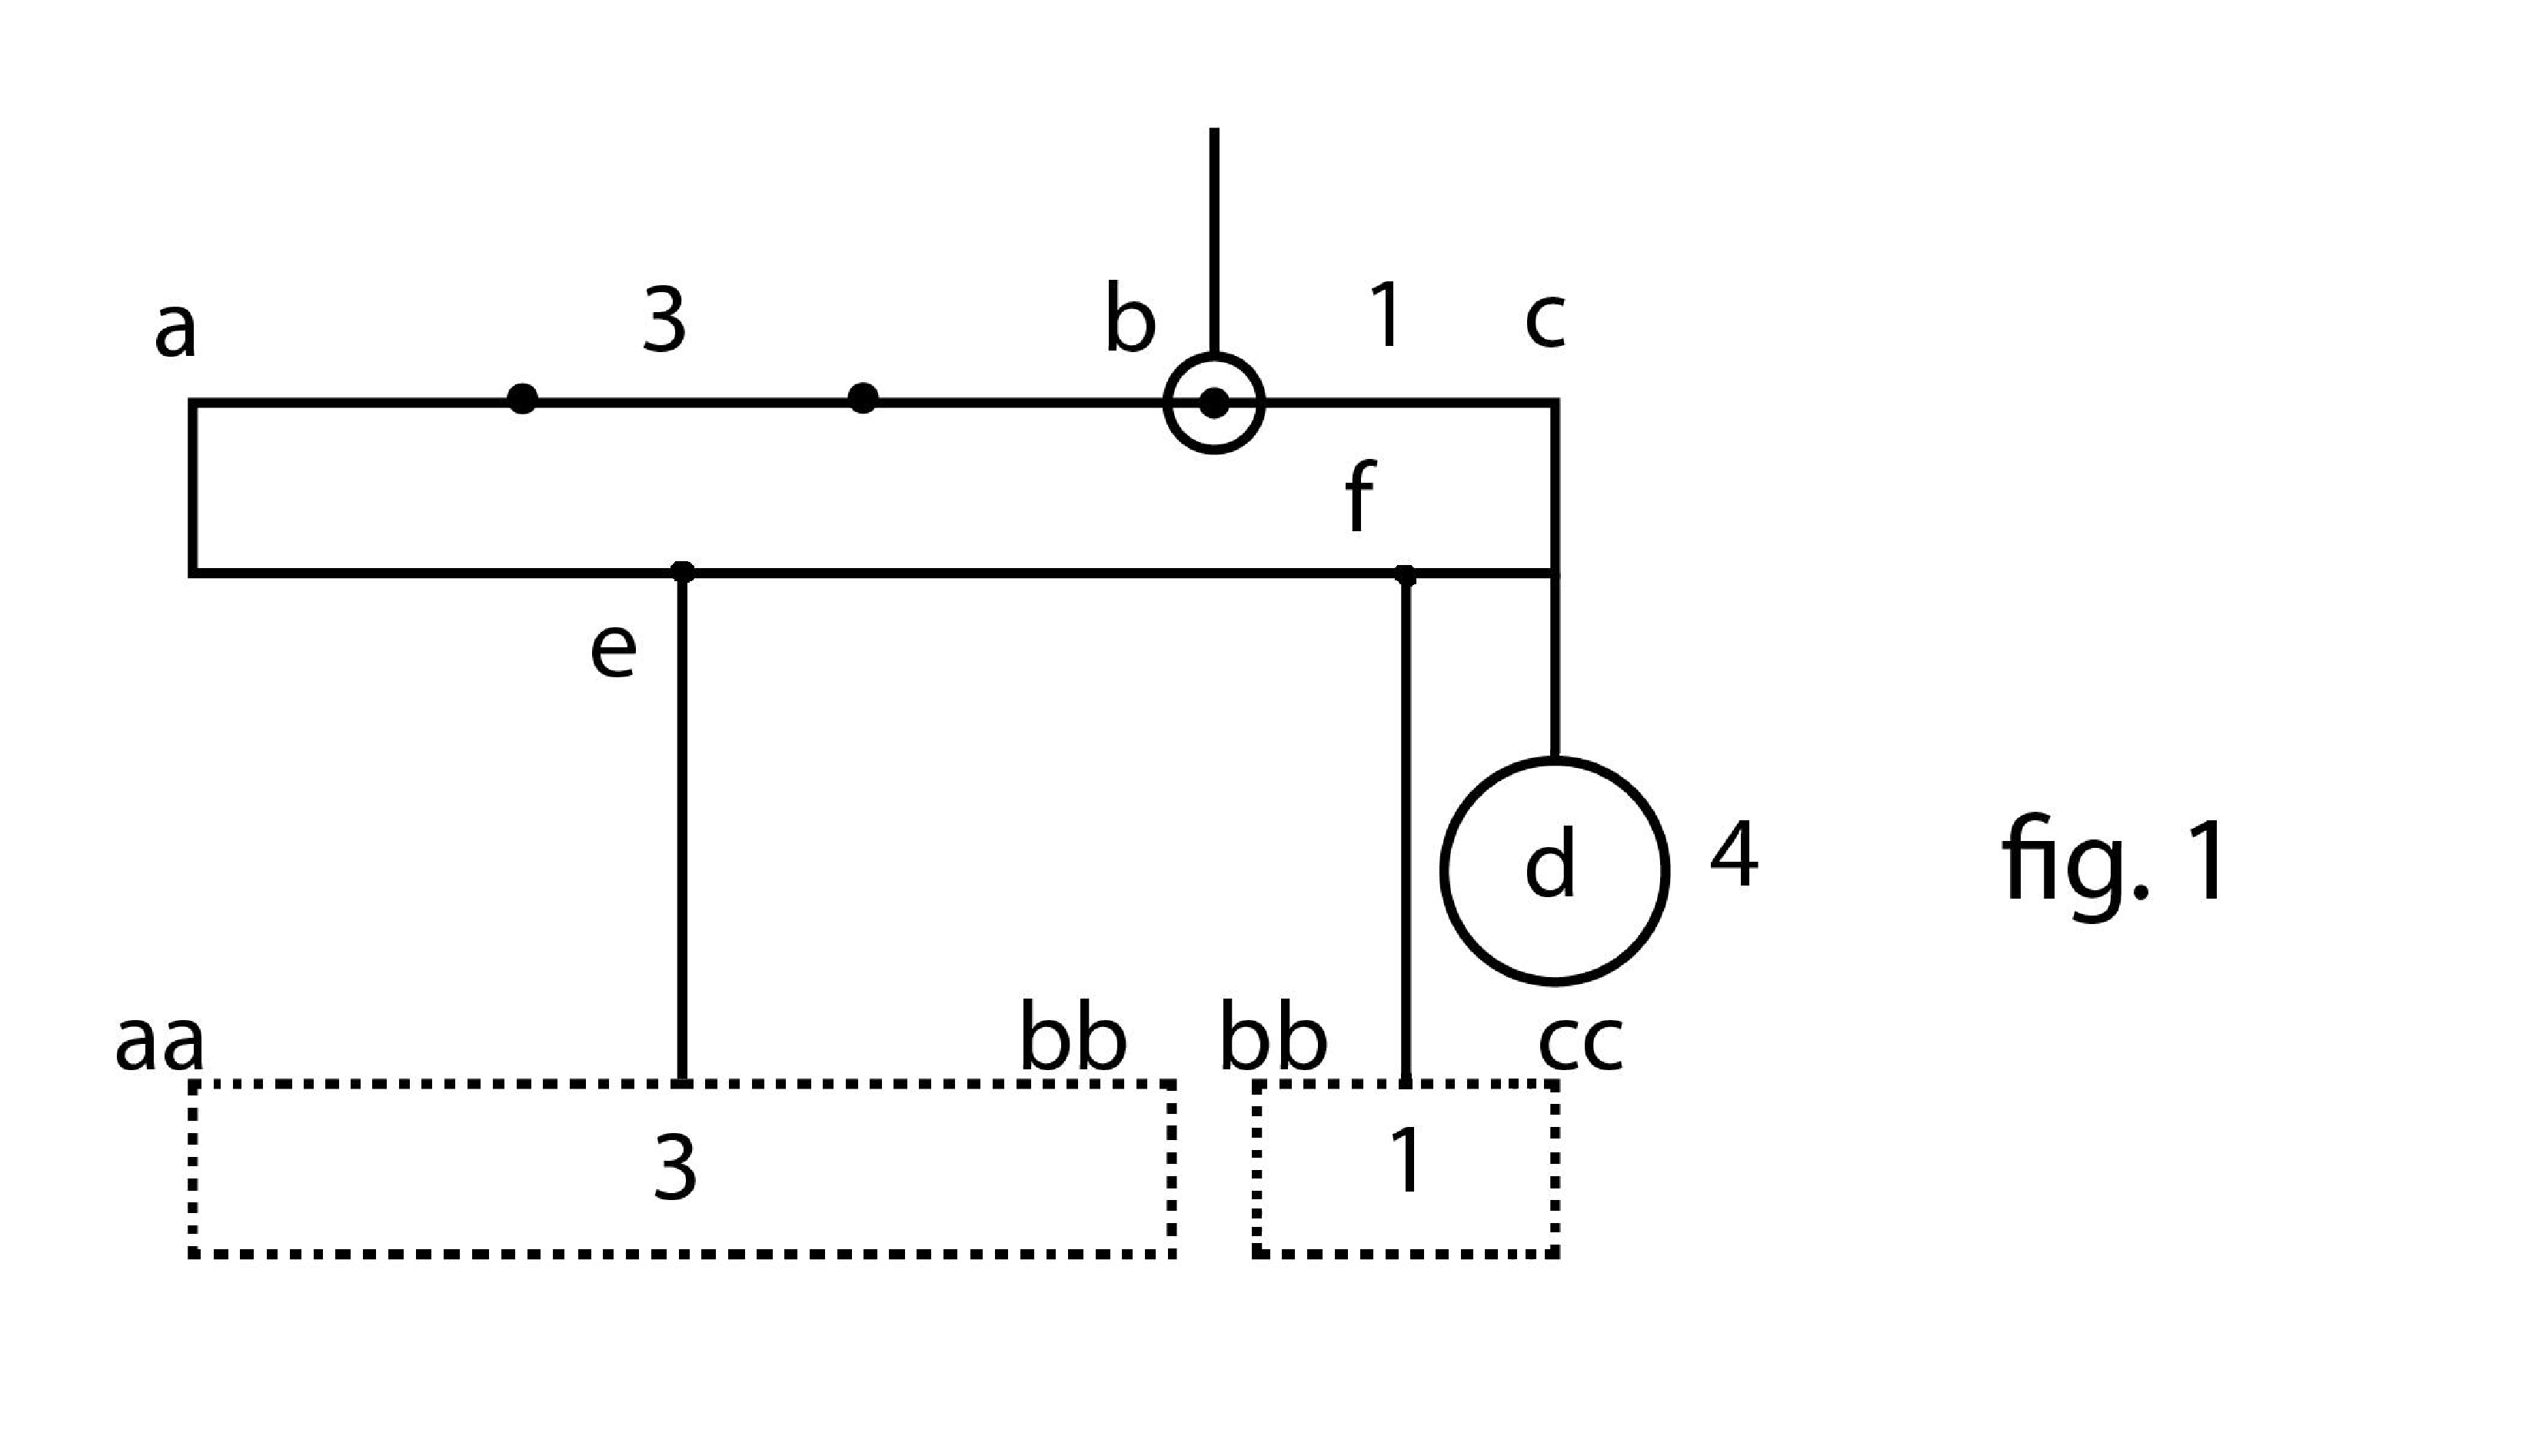
\includegraphics[trim = 0mm 22mm 0mm 0mm, clip, width=0.5\textwidth]{images/LH037,05_135-d1.pdf}\\
%% \noindent \centering[\textit{Fig. 1}] 
%\end{wrapfigure}%
\noindent%
[135~r\textsuperscript{o}] 
\edtext{Si corpus}{\lemma{Si}\Bfootnote{\textit{(1)}\ sit \textit{(2)}\ corpus \textit{L}}} cylindricum,\edtext{}{\lemma{}\killnumber\Afootnote{\textit{Am Rand unter} fig. 1:
Haec cum scriberem nondum intelligebam quid esset centrum Gravitatis.\protect\index{Sachverzeichnis}{centrum gravitatis}\vspace{-6mm}}} (: quale est Cylinder, Rectangulum Solidum, aliaque corpora,
quae fiunt ex ductu basis in altitudinem~:)  $abc$ \edtext{suspensum sit ex}{\lemma{}\Bfootnote{suspensum\ \textbar\ sit \textit{erg.}\ \textbar\ ex \textit{ L}}} centro $b$ ita ut brachium\protect\index{Sachverzeichnis}{brachium} $ab$ sit majus, $bc$ minus \edtext{in ratione cognita}{\lemma{}\Bfootnote{in ratione cognita \textit{erg.} \textit{L}}}; invenire pondus\protect\index{Sachverzeichnis}{pondus} $d$, quo appenso ex puncto $c$ brachium\protect\index{Sachverzeichnis}{brachium} $bc$ sit in aequilibrio\protect\index{Sachverzeichnis}{aequilibrium} cum brachio $ab$.\\
\indent Id quidem tam facile est, ut compendiosas artes quaerere non sit operae pretium. 
\pend
\pstart
Esto $bc$ librae\protect\index{Sachverzeichnis}{libra} unius, $ba$ trium, centrum  gravitatis\protect\index{Sachverzeichnis}{centrum gravitatis} $ab$ in medio $e$ et centrum gravitatis\protect\index{Sachverzeichnis}{centrum gravitatis} $bc$\hfill in\hfill medio\hfill $f$.\hfill Ergo\hfill si\hfill $ab$\hfill vel\hfill  $aabb$\hfill suspensum\hfill intelligeretur\hfill ex\hfill $e$\hfill \edtext{et\hfill $bc$\hfill ex\hfill $f$}{\lemma{}\Bfootnote{et $bc$ ex $f$ \textit{erg.} \textit{L}}}\hfill tantundem
\pend
\vspace{1em}
\pstart
\centering
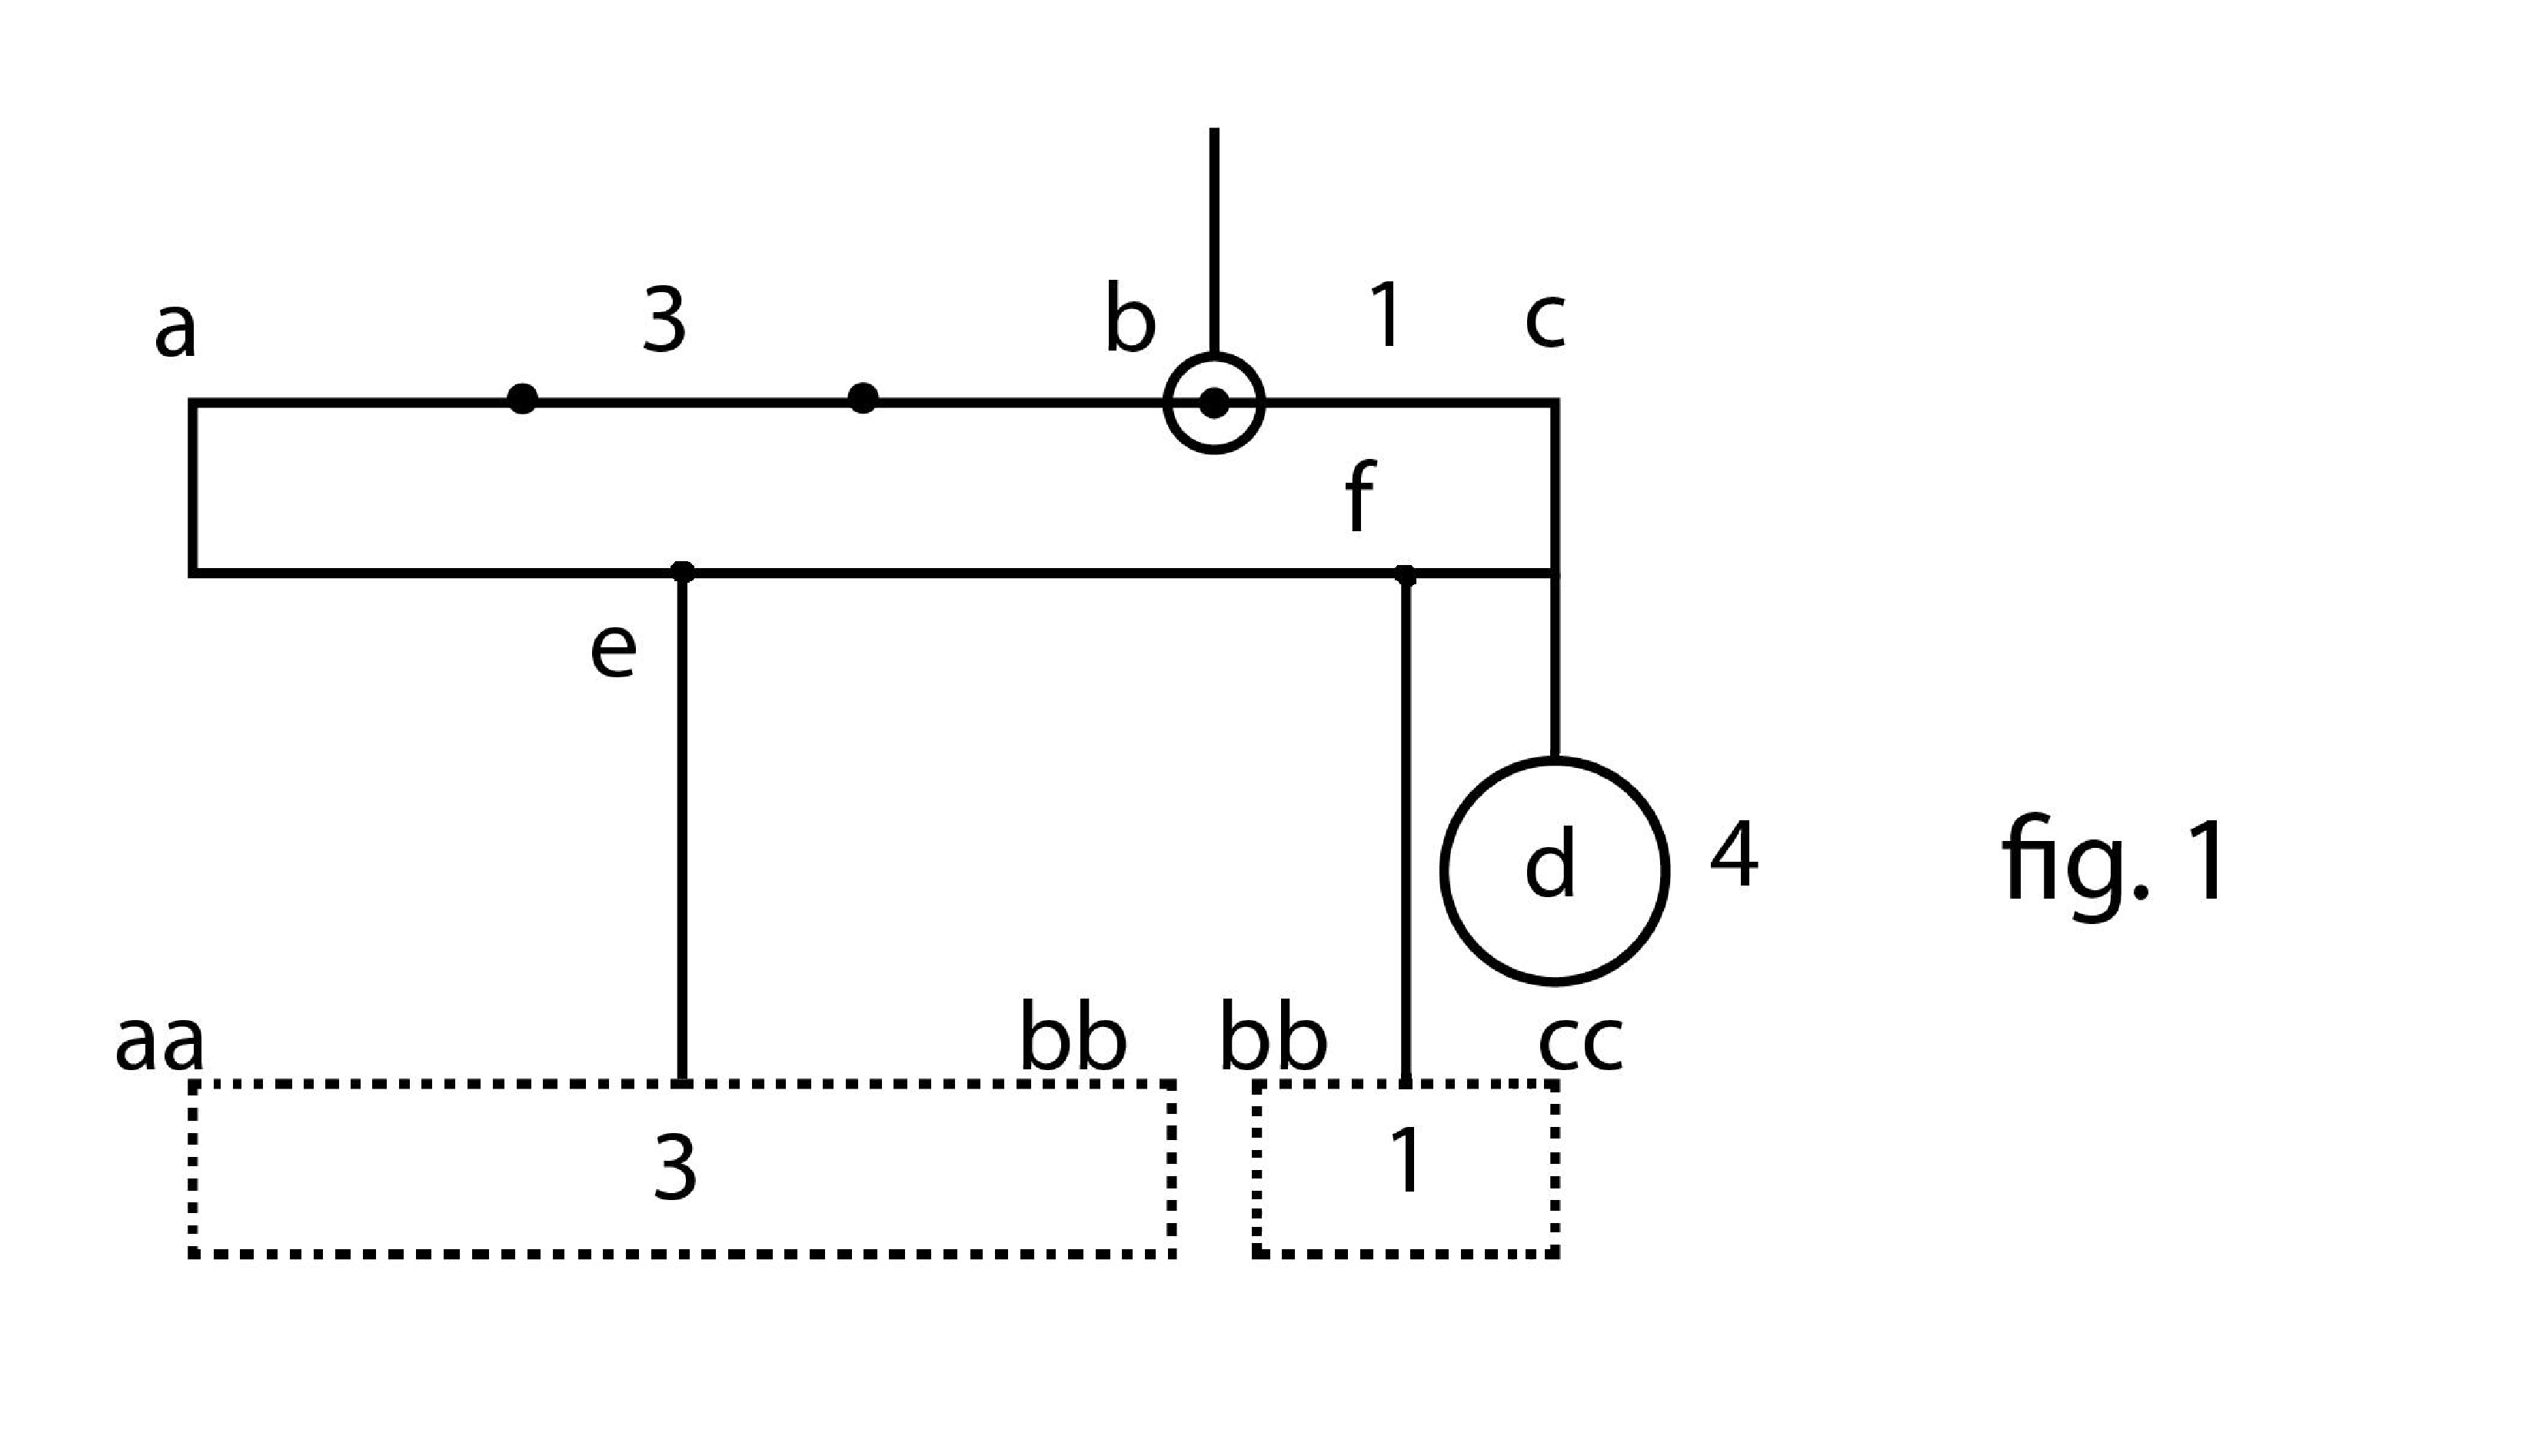
\includegraphics[trim = -30mm 22mm 0mm 0mm, clip, width=0.55\textwidth]{images/LH037,05_135-d1.pdf}
\pend
\newpage
\count\Afootins=1200
\count\Bfootins=1200
\count\Cfootins=1200
\pstart \noindent gravitarent, quantum nunc cum centrum $b$ attingunt. Porro $be$ est triplum $bf$. Ergo si $bbcc$ ex $f$ valet unam libram\protect\index{Sachverzeichnis}{libra}, $aabb$ ex $e$ (cujus distantia a centro $b$ triplo major est) valebit libras\protect\index{Sachverzeichnis}{libra} novem. Ergo 8 librae \edtext{ex \textit{bf}}{\lemma{}\Bfootnote{ex \textbar\ centro \textit{gestr.}\ \textbar\ $bf$ \textit{L}}} appendendae essent, ut $bc$ aequivaleat ipsi $ab$. Sed cum ex duplo \textit{bf} nempe ex $bc$ suspendendae sint, sufficiunt librae 4\protect\index{Sachverzeichnis}{libra}. 
\pend
\pstart
Erit ergo pondus\protect\index{Sachverzeichnis}{pondus} $d$ librarum 4\protect\index{Sachverzeichnis}{libra}, quod erat inveniendum. Eodem modo facile est per regressum dato pondere\protect\index{Sachverzeichnis}{pondus} $d$ et cylindrico $ac$ invenire punctum suspensionis $b$ ut fiat brachiorum aequilibrium\protect\index{Sachverzeichnis}{aequilibrium brachiorum}. 
\pend 
\pstart
\vspace*{1em}
\begin{minipage}[t]{0.5\textwidth}
\hspace{-9mm}
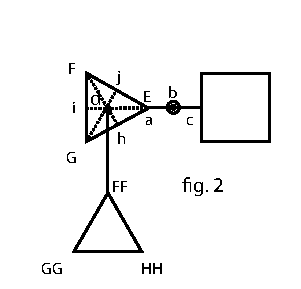
\includegraphics[width=0.75\textwidth]{images/LH037,05_135-d2.pdf}
%\noindent \centering [\textit{Fig. 2}] 
\end{minipage}
\hspace{1mm}
\begin{minipage}[t]{0.5\textwidth}
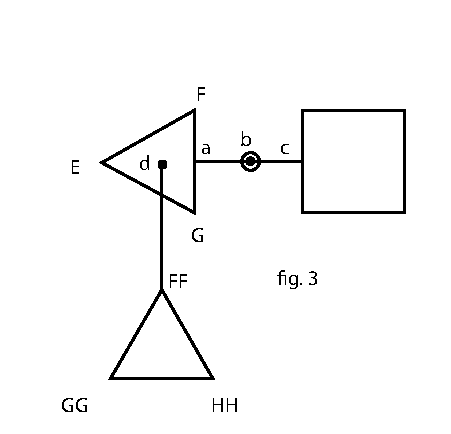
\includegraphics[width=0.85\textwidth]{images/LH037,05_135-d3.pdf}
%\noindent \centering [\textit{Fig. 3}] 
\end{minipage}
   \pend
    \vspace{1.5em} 
\pstart
Sed \setline{8}ista Methodus\protect\index{Sachverzeichnis}{methodus}, (qua corpus supponitur suspendi ex suo centro gravitatis\protect\index{Sachverzeichnis}{centrum gravitatis}) non est universalis, quod exemplo ostendo. Esto in fig. 2 Triangulum aequilaterum $EFG$ infixum apice $E$ in brachio\protect\index{Sachverzeichnis}{brachium} $ab$ quod continuatum incideret in $d$ centrum gravitatis\protect\index{Sachverzeichnis}{centrum gravitatis} Trianguli.
\newline%
\indent%
Supponatur latus Trianguli aequilateri esse 3.
\protect\rule[-4mm]{0mm}{10mm}%
Erit altitudo $Fdh$, Rq, \edtext{$\displaystyle 9-\frac{9}{4}$. Area}{\lemma{$\displaystyle 9-\frac{9}{4}$.}\Bfootnote{\textit{(1)}\ Summa \textit{(2)}\ Area \textit{L}}} $\displaystyle \bigtriangledown^{li}$ est Rq $\displaystyle\frac{27}{4}$ ducta in 3. \edtext{seu Rq 9.}{\lemma{seu Rq 9.}\Bfootnote{\textit{erg.} \textit{L}}} \edtext{producto dimidiato}{\lemma{producto dimidiato}\Bfootnote{\textit{gestr. u. wieder gültig gemacht} \textit{L}}} \edtext{fiet Rq,$\displaystyle\frac{27\smallfrown9}{8}$}{\lemma{fiet}\Bfootnote{\textit{(1)}\ Rq,$\displaystyle\frac{27\smallfrown9}{4}$ \textit{(2)}\ Rq,$\displaystyle\frac{27\smallfrown9}{8}.$ \textit{L}}}\edtext{.}{\lemma{Rq,$\displaystyle\frac{27\smallfrown9}{8}$}\Cfootnote{Leibniz ersetzt nicht durchgegend die 4 im Nenner durch 8. Die richtige Zahl im Nenner beträgt 16. Der Fehler wirkt sich auf die nachfolgenden Rechnungen des Stückes aus.}} Erit Area Trianguli Rq: \protect\rule[-4mm]{0mm}{10mm}$\displaystyle\frac{243}{8}$.
[135~v\textsuperscript{o}]
\pend 
\newpage
\pstart
Jam ut inveniatur centrum gravitatis\protect\index{Sachverzeichnis}{centrum gravitatis} $d$ seu recta $Ed$, et recta $dh$ resolvi intelligatur hoc triangulum in tria triangula  isoscelia, inter se aequalia \textit{FdG}, \textit{GdE}, \textit{EdF}. Et unius eorum ut $GdE$ area erit tertia pars areae \protect\rule[-4mm]{0mm}{10mm}totius \edtext{Trianguli Rq. $\displaystyle \frac{243}{8}$.}{\lemma{}\Bfootnote{Trianguli\ \textbar\ Rq. $\displaystyle60\frac{3}{4}$ \textit{gestr.}\ \textbar\ vel \textit{streicht Hrsg.}\ \textbar\ Rq.$\displaystyle\frac{243}{8}$. \textit{L}}}
 Dividatur ergo area per 3. seu Rq 9. Fiet  Rq $\displaystyle\frac{27}{8}$ area Trianguli $GdE$ quae alioquin etiam fit ex ductu basis \edtext{dimidiae}{\lemma{}\Bfootnote{dimidiae \textit{erg.} \textit{L}}} $GE$ in altitudinem $dh$. Ergo \edtext{vice versa}{\lemma{}\Bfootnote{vice versa \textit{erg.} \textit{L}}} si Rq \protect\rule[-4mm]{0mm}{10mm}$\displaystyle\frac{27}{4}$ area Trianguli $GdE$ dividatur per \edtext{dimidiam}{\lemma{}\Bfootnote{dimidiam \textit{erg.} \textit{L}}} basin $GE$ $\displaystyle\frac{3}{2}$ seu Rq$\displaystyle \frac{9}{4}$. Habebimus $\displaystyle\frac{27}{5}\bigtimes\frac{9}{4}$  $\displaystyle \frac{27}{9}\bigg \vert3$. Facit Rq 3. pro \edtext{[$dh$]}{\lemma{}\Bfootnote{\textit{da} \textit{\ L \"{a}ndert Hrsg.}}} quae si auferantur ex $Fh$ altitudine, quae est Rq \protect\rule[-4mm]{0mm}{10mm}$\displaystyle \frac{27}{4}$. Erit $Ed$ distantia centri gravitatis\protect\index{Sachverzeichnis}{centrum gravitatis} \edtext{$d$}{\lemma{}\Bfootnote{$d$ \textit{erg.} \textit{L}}} a puncto suspensionis $a$ in figura \edtext{[secunda]}{\lemma{prima}\Bfootnote{\textit{L \"{a}ndert Hrsg.}}}
\edtext{Rq $\displaystyle\frac{27}{4}-$ Rq 3.
\newline%
\indent$ab$ esto}{\lemma{Rq $\displaystyle\frac{27}{4}-$ Rq 3.}\Bfootnote{\textit{(1)}\ $ab$ distantia \textit{(2)}\ $ab$ esto \textit{L}}} \edtext{etiam}{\lemma{}\Bfootnote{etiam \textit{ erg.} \textit{ L}}} Rq 3. Erit in fig. \edtext{[2.]}{\lemma{}\Bfootnote{1.\textit{\ L \"{a}ndert Hrsg.}}} $bEd$ Rq\protect\rule[-4mm]{0mm}{10mm}$\displaystyle\frac{27}{4}$. Gravitabit ergo Triangulum ex Rq$\displaystyle\frac{27}{4}$. 
\pend
\pstart
At in fig. \edtext{[3.]}{\lemma{}\Bfootnote{2.\textit{\ L \"{a}ndert Hrsg.}}} gravitabit \edtext{\textit{bad}[,] componetur}{\lemma{}\Bfootnote{\textit{bad}[,] \textbar\ quae \textit{gestr.}\ \textbar\ componetur \textit{L}}} ex $ba$ Rq 3 et $ad$ Rq 3. Erit summa $bad$~Rq~$\displaystyle3\smallfrown$ Rq~\protect\rule[-4mm]{0mm}{10mm}$\displaystyle\frac{4}{1}$
\edtext{seu Rq 12.
\newline% 
\indent%
Ergo}{\lemma{seu Rq 12.}\Bfootnote{\textit{(1)}\ vel Rq 3. \textit{(2)}\ Ergo \textit{L}}} ut est Rq. 12 ad Rq~$\displaystyle\frac{27}{4}$ ita \edtext{erit, admissa}{\lemma{erit,}\Bfootnote{\textit{(1)}\ ex \textit{(2)}\ admissa \textit{L}}}
ex hypothesi calculi centri gravitatis\protect\index{Sachverzeichnis}{centrum gravitatis}, Triangulum $EFG$ in fig. 3. ad idem in fig. 2\textsuperscript{da}. Seu Ratio erit Rq~\protect\rule[-4mm]{0mm}{10mm}$\displaystyle\frac{\displaystyle\frac{27}{4}}{12}$ seu Rq~$\displaystyle\frac{27}{48}\bigg \vert\frac{9}{16}$ seu $\displaystyle\frac{3}{4}$.
\pend
%\vspace{1.5em}
\pstart
Esto in fig. 4. idem Triangulum $EFG$ et linea  $bai$ quae in \edtext{fig. 2. Esto et}{\lemma{fig. 2.}\Bfootnote{\textit{(1)}\ intelligatur \textit{(2)}\ Esto et\textit{ L}}} rectangulum, $IFmG$, cujus longitudo $bai$ latitudo $FG$ fiat in fig. 5. Triangulum rectangulum, cuius altitudo $bai$ basi parallela in $a$ sit $FG$. Erit Rectangulum $iFG$ fig. 5 simile et aequale rectangulo\hfill $oFG$\hfill fig.\hfill 4.\hfill repraesentabitque\hfill eius\hfill pondus\protect\index{Sachverzeichnis}{pondus}\hfill absolutum,\hfill at Trapezium\hfill $iFGn$
\pend
\pstart
\begin{minipage}[t]{0.5\textwidth}
\hspace{-9mm}
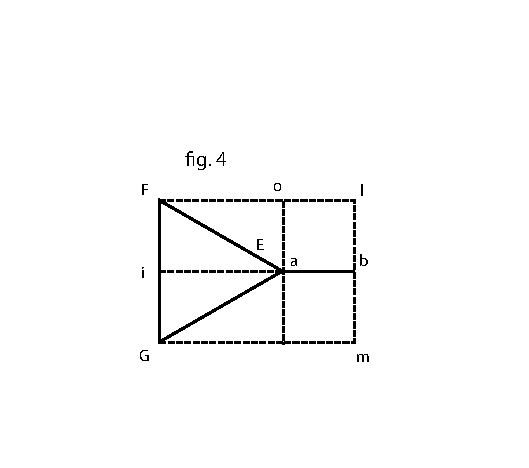
\includegraphics[width=0.74\textwidth]{images/LH037,05_135-d4.pdf}
%\noindent \centering [\textit{Fig. 4}]
\end{minipage}
\hspace{11mm}
\begin{minipage}[t]{0.5\textwidth}
%\hspace*{5mm}
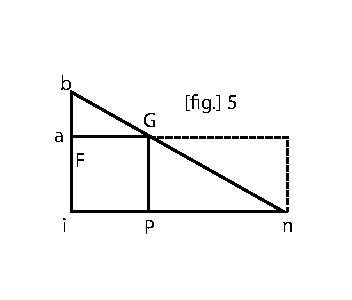
\includegraphics[width=0.72\textwidth]{images/LH037,05_135-d5.pdf}
%\noindent \centering [\textit{Fig. 5}]
\end{minipage}
%\hspace*{17,3mm}
%\begin{minipage}[t]{0.2\textwidth}
%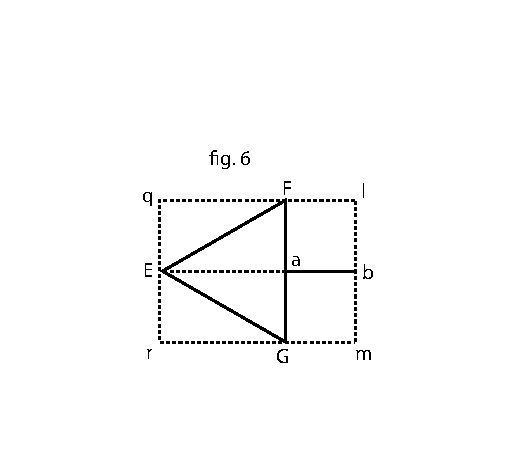
\includegraphics[width=1\textwidth]{images/LH037,05_135-d6.pdf}
%%\noindent \centering [\textit{Fig. 6}]
%\end{minipage}
%\vspace*{0.5em}
\pend
\count\Bfootins=1200
\vspace{1.5em}
\pstart\noindent \edtext{fig. 5.}{\lemma{}\Bfootnote{fig. 5. \textit{erg.} \textit{L}}} \setline{1}repraesentabit potentiam seu gravitationem Rectanguli $oFG$ ex centro $b$ fig. 4. et totum Triangulum $bin$ fig. 5.
[136~r\textsuperscript{o}]
repraesentat gravitationem totius rectanguli $lFG$  ex centro $b$. Quaeritur jam quomodo exhibeatur potentia seu gravitatio rectanguli $EFG$ 
\edtext{fig. 4.}{\lemma{}\Bfootnote{fig. 4. \textit{erg.} \textit{L}}} 
ita ut $E$ sit infixum in brachio\protect\index{Sachverzeichnis}{brachium} $a$. Id ita fiet: investigemus tantum potentiam seu gravitationem dimidii ejus $EiF$ \textso{fig. 4.} Id ita fiet: Triangulum $EiF$ vel $aiF$ \textso{fig. 4.} intelligatur locari erectum super $ai$ \textso{figurae 5\textsuperscript{tae}} atque ita duci intelligatur in Trapezium fig. 5. $iFGn$. Productum  
\edtext{solidum repraesentabit}{\lemma{solidum}\Bfootnote{\textit{(1)}\ erit \textit{(2)}\ repraesentabit \textit{L}}} 
potentiam Trianguli \textit{aif}. Quod solidum ita computabimus: $ai$
\edtext{\textso{fig. 5.}}{\lemma{\textso{fig.}}\Bfootnote{\textit{(1)}\ \textso{4} \textit{(2)}\ \textso{5} \textit{L}}} est Rq \protect\rule[-4mm]{0mm}{10mm}$\displaystyle\frac{27}{4}$[,] $FG$ est 3. \edlabel{LH-Nummer_LH037_05_135-136_a1}Factum ex ipsis Rq \protect\rule[-4mm]{0mm}{10mm}$\displaystyle\frac{243}{4}$ area Rectanguli $iFG$. Hoc ducatur in $iF$ Rq $\displaystyle\frac{27}{8}$ fiet Rq $\displaystyle\frac{6561}{32}$ cujus dimidium est Rq $\displaystyle\frac{6561}{128}$. Jam ut est $ba$ Rq 3. ad $FG$ 3. ita est  $GP$ vel $ai$ Rq \protect\rule[-4mm]{0mm}{10mm}$\displaystyle\frac{27}{4}$ ad $Pn$. Erit Rq $\displaystyle\frac{27}{4}\efrac{-}{-}$Rq $\displaystyle\frac{9}{1}=$ Rq \protect\rule[-4mm]{0mm}{10mm}$\displaystyle\frac{243}{4}\bigtimes$ Rq $\displaystyle\frac{3}{1}$= Rq $\displaystyle\frac{243}{12}$. 
Ducatur in $ai$ Rq $\displaystyle\frac{27}{4}\efrac{-}{-}$Rq $\displaystyle\frac{243}{12}=$
\edtext{Rq $\displaystyle\frac{6561}{48}\bigg\vert^{\underset{\smile}3}\frac{2187}{16}.$ 
Hoc ducatur in $iF$ Rq $\displaystyle\frac{27}{8}\efrac{-}{-}$Rq $\displaystyle\frac{2187}{16}.$}{%
\lemma{Rq $\displaystyle\frac{6561}{48}\bigg \vert^{\protect\underset{\smile}3}\frac{2187}{16}.$}%
\Bfootnote{ \textit{(1)}\ Unius dimidium Rq $\displaystyle\frac{2187}{64}$\
\textit{(2)}\ Hoc ducatur in $iF$ Rq $\displaystyle\frac{27}{8}\efrac{-}{-}$Rq $\displaystyle\frac{2187}{16}.$ \textit{ L}}}
\protect\rule[-4mm]{0mm}{10mm}productum dividatur per 4. seu
\edtext{Rq 16.
Sed tamen et rursus duplicetur ob duplum triangulum \textit{iFE} fig. 4. manebit:}{\lemma{}%
\Bfootnote{Rq 16.\ \textbar\ Sed [...] fig. 4. \textit{erg.}\ \textbar\ \textit{(1)}\ fiet \textit{(2)}\ manebit: \textit{ L}}}
Rq $\displaystyle\frac{27}{8}\efrac{-}{-}\displaystyle\frac{2187}{16}=\displaystyle\frac{59094}{128}.$%
\edlabel{LH-Nummer_LH037_05_135-136_a2}
Addantur in unum: \protect\rule[-4mm]{0mm}{10mm}Rq 6561\,+\,Rq\,$\displaystyle \frac{59094}{128}$.
Productum erit summa potentiae Trianguli
\edtext{$EFG.$}{\lemma{\hspace{1.8mm}2f. \hspace{1.8mm}$EFG.$}\killnumber\Bfootnote{\textit{(1)}\ Sed inver \textit{(2)}\ Sed si inversum \textit{L}}}
\pend
\vspace{1mm}
\pstart% 
\begin{window}[0,r,\hspace{2mm}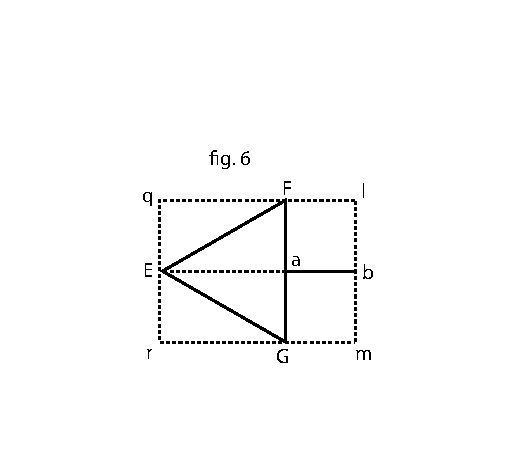
\includegraphics[%trim = -3mm -2mm 0mm 0mm, clip,
width=0.3\textwidth]
{images/LH037,05_135-d6.pdf}, {}]
\indent
Sed si inversum intelligatur Triangulum, Basi $FG$ versus Centrum vectis 
\edtext{$b$}{\lemma{4 \hspace{1.8mm}$b$}\killnumber\Bfootnote{\textit{erg. L}}} 
convexa, ut in fig. 6. ubi $ba$ incidit
\edtext{perpendiculariter}{\lemma{5}\killnumber\Bfootnote{perpendiculariter \textit{erg. L}}} 
{in\reversemarginpar\marginnote{\scriptsize\hspace{-13mm}5}} mediam $FG.$
Ducendum quidem rursus est in Trapezium $iaGn$ \textso{fig. 5.}
dimidium trianguli $EFG.$
nempe $EiF$ fig. 4.
aut $aEF$\textso{ fig. 6.} sed eo discrimine,
quod altitudo Trianguli $iF$ (fig. 4) insistere debet ipsi $a$\textso{ figurae 5.} et apex $E$ %
\edtext{\textso{fig. 4.}}{\lemma{9 \hspace{1.8mm}\textso{fig. 4.}}\killnumber\Bfootnote{\textit{ erg. L}}}
ipsi $i$ fig. 5.
Ita producetur quidem idem quod ante {rectangulum\reversemarginpar\marginnote{\scriptsize\hspace{-13mm}10}} $FGP$ fig. 5. nempe Rq \protect\rule[-4mm]{0mm}{10mm}$\displaystyle\frac{6561}{32}$.
\end{window}
\pend
%\newpage
\vspace{2em}
\pstart
\noindent\lbrack\textit{Nebenrechnungen am Rand zu S. \refpassage{LH-Nummer_LH037_05_135-136_a1}{LH-Nummer_LH037_05_135-136_a2}:}\rbrack\setline{6}
\pend
\pstart
\vspace*{1em}
\begin{minipage}[t]{0.2\textwidth}
\hspace*{-5mm}
$\begin{array}{ll}
&\ ~243\\
&\uline{\quad27}\\
&1701\\ 
&\uline{486~ \ }\\
&\displaystyle\frac{6561}{32\ ~} \bigg \vert \\
\end{array}$
\end{minipage}
\hspace*{17,3mm}
\begin{minipage}[t]{0.2\textwidth}
$\begin{array}{ll}
&\ 2187\\
&\uline{\quad~27}\\
&15309\\ 
&\uline{4374 \ }\\
&59049\\
\end{array}$
\end{minipage}
\pend
\vspace{1.5em}
\pstart
\noindent
\lbrack%
\textit{Gestrichene Rechnung dazu:}\edtext{}{\lemma{\: \lbrack\textit{Gestrichene Rechnung}\rbrack}\killnumber\Cfootnote{Der Radikand ist zu hoch angesetzt. Der richtige ganzzahlige Bestandteil des Radikanden ist 46.}}%
\rbrack
\hspace*{17,3mm}
\begin{minipage}[t]{0.2\textwidth}
\hspace*{-5mm}
\edlabel{LH-Nummer_LH037_05_135-136_b1}
$\begin{array}{ll}
&\ \cancel{1}\\
&\ \cancel{5}\ 4\\
&\cancel{2}\cancel{\underset{\cdot}1}\cancel{8}\underset{\cdot}7\\
&\overline{\ \, 4 \ \, 8 \ }\\
&\overline{1\cancel{6}\cancel{8}8}\\
\end{array}$
\end{minipage}
\pend
\count\Afootins=1500
\count\Bfootins=1500
\count\Cfootins=1500